\documentclass[14pt,aspectratio=169,hyperref={pdftex,unicode},xcolor=dvipsnames]{beamer}
\usepackage[english,russian]{babel}
\usepackage[utf8x]{inputenc}
\usepackage[T2A]{fontenc}
\usepackage{cmap}
\usepackage{paratype}
\usepackage{minted} % для примеров кода (требует параметра -shell-escape)

\usetheme{metropolis}
\usefonttheme[]{professionalfonts}  % запрещаем beamer'у перезаписывать мат. шрифты
\metroset{numbering=fraction}
\metroset{subsectionpage=progressbar}

\setbeamercolor{frametitle}{fg=black}
\setbeamertemplate{frametitle}
{
 \vspace{3mm}\insertframetitle\par
}
\setbeamertemplate{title separator}{}
\setbeamertemplate{footnote separator}{}


\usebackgroundtemplate{
\includegraphics[width=\paperwidth,height=\paperheight]{./common/background_white.jpg}}

\logo{\vspace{-1.2cm}
\includegraphics[width=6mm]{./common/short-v.pdf}\hspace*{1.08\textwidth}}

\institute
{
  \begin{columns}
    \begin{column}{1.5cm}
    
\includegraphics[height=15mm,keepaspectratio]{./common/math-cs.pdf}
    \end{column}
    \begin{column}{4cm}
          Факультет математики и компьютерных наук СПбГУ
    \end{column}
  \end{columns}
}


\begin{document}

\begin{frame}[plain]
  \begin{center}
    \textbf{Имя и фамилия автора}

    {\Large\textbf{Тема работы: довольно длинное название строки на две минимум}}

    Выпускная квалификационная работа

    {\small Научный руководитель: А.\,А.\,Выбегалло}

    ДАТА ЗАЩИТЫ
  \end{center}


  \begin{columns}
    \begin{column}{1cm}
    
\includegraphics[height=15mm,keepaspectratio]{./common/math-cs.pdf}
    \end{column}
    \begin{column}{10cm}
      \small
          Факультет математики и~компьютерных наук СПбГУ\\
          Программа <<Современное программирование>>
    \end{column}
  \end{columns}
\end{frame}



\begin{frame}
\frametitle{Введение в предметную область}

\begin{itemize}
\item О чём здесь вообще речь? Для чего вообще этим всем стоит заниматься?
\item В чём актуальность работы?
\item Кто ещё этим занимается, с кем мы будем сравниваться?
\item Этот слайд необходим для того, чтобы постановка задачи была понятнее.
\item Вряд ли стоит делать больше двух таких слайдов, иначе вы не успеете рассказать о своей работе.
\item На введение в предметную область должно уйти не более 15\% времени вашего доклада.
\end{itemize}


\end{frame}

\begin{frame}
\frametitle{Постановка задачи}
\begin{enumerate}
\item Разработать алгоритм решения задачи путешествующего сейлсмена\footnote{Крайне рекомендуется избегать англицизмов --- старайтесь использовать принятые в~русском языке термины.}, работающий за полиномиальное время.
\item Построить программную implementation\footnote{Так тоже не надо.}, протестировать её~производительность и сравнить с конкурентами.
\item Оформить результаты работы в виде доклада на~STOC\footnote{Злоупотреблять аббревиатурами также не стоит, используйте только действительно общепринятые и всем известные сокращения.}.
\end{enumerate}
\end{frame}

\begin{frame}{Задача 1: формула с пояснениями}
\small
    Фильтр минимизирует среднеквадратическое отклонение цвета пикселя.
    
    \begin{equation*}\label{eq:wiener_nsr}
    \hat{Y}(i, j) = \left[ \frac{\hat{H}^*(i, j)}{\left|\hat{H}(i, j)\right|^2 + \frac{S_n(i, j)}{S_s(i, j)}} \right] \times \hat{F}(i, j),
    \end{equation*}
\begin{itemize}
    \item $Y$ -- восстановленное изображение,  $F$ -- наблюдаемое изображение,
    \item $H$ -- функция рассеивания, $H^*$ --комплексное сопряжение $H$,
    \item $S_n$ -- энергетический спектр шума -- $\left| \hat{N} \right|^2$,
    \item $S_s$ -- энергетический спектр исходного изображения -- $\left| \hat{F} \right|^2$,
    \item $\times$ -- умножение комплексных чисел.
\end{itemize}
\end{frame}


\begin{frame}[fragile]
\frametitle{Задача 2: код на языке программирования\footnote{Увлекаться кодом на слайдах не стоит, зато структурные и иные диаграммы обычно смотрятся хорошо.}}
\begin{minted}{kotlin}
fun main() {
    val name = "stranger"
    println("Hi, $name!")
    print("Current count:")
    for (i in 0..10) {
        print(" $i")
    }
}
\end{minted}
\end{frame}

\begin{frame}{Задача 2: результаты измерений в таблице}
\centering
\begin{tabular}{lccc}
    Имя & Работа 1 & Работа 2 & Итог \\
\hline\hline
    Алиса & 8.0 & 9.0 & 8.5 \\
    Боб & 9.0 & 9.8 & 9.4 \\
    Чак & 9.1 & 9.3 & 9.2 \\
\end{tabular}

\begin{block}{Пояснения к таблице}
  \begin{itemize}
  \item Таблицы могут требовать пояснений.
  \item Что это за величины? Откуда они взялись?
  \item Какие выводы можно сделать?
  \end{itemize}
\end{block}

\end{frame}


\begin{frame}
\frametitle{Задача 2: результаты сравнения с конкурентами\footnote{Понятна ли ваша диаграмма? Не забыли ли вы легенду?}\footnote{Контрастно ли изображение? Помните, на проекторе всё может выглядеть хуже.}}
\begin{center}
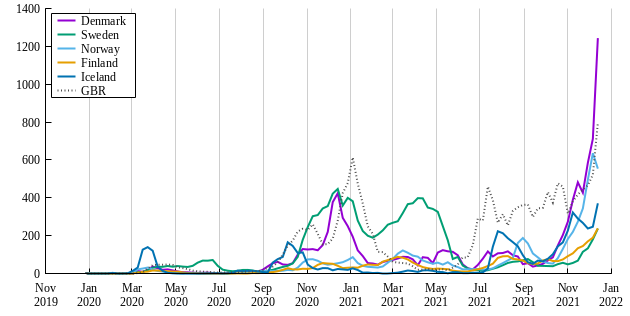
\includegraphics[width=11cm]{images/graph.png}
\end{center}
\end{frame}

\begin{frame}
\frametitle{Задача 3: основные трудности}
\begin{itemize}
\item Мы всё классно сделали, но рецензенты STOC сформулировали ряд претензий к~работе, обозвали нас идиотами и отказались пускать на конференцию.
\item Все замечания были исправлены, попробуем FOCS\footnote{Не забывайте про нежелательность англицизмов и аббревиатур.}!
\end{itemize}

\end{frame}

\begin{frame}
\frametitle{Дополнительный слайд по работе в целом\footnote{Кстати, слайды с длинными перечислениями выглядят плохо. Старайтесь их избегать.}}
\begin{itemize}
\item Освоенные и применённые технологии
\item Информация о внедрении
\item Полученные в ходе выполнения работы навыки
\item Вынесенные уроки
\item Реальные планы на будущее (не надо фантазировать!)
\item Ссылки на цитированную литературу --- их можно вынести в конец слайдов, но во время доклада не показывать.
\end{itemize}

\end{frame}


\begin{frame}
\frametitle{Результаты работы}

\begin{enumerate}
\item Разработан полиномиальный алгоритм решения задачи коммивояжёра.
\item Программная реализация демонстрирует высочайшую производительность и превосходит все известные аналоги.
\item Результаты подготовлены для представления на~FOCS.
\end{enumerate}

\vspace{5mm}\hrule\vspace{5mm}

\begin{center}
Имя, фамилия и контакты автора,\\ссылка на материалы работы, QR-код.
\end{center}

\end{frame}

\begin{frame}[noframenumbering,plain]
\frametitle{}
\begin{center}
  \Huge Спасибо за внимание!

  Ваши вопросы?

  {\color{red}Этот слайд не нужен! Удалите его\footnote{Сноски на слайдах тоже удалите: не нужно усложнять их структуру и содержимое. Не~забывайте, что многое можно просто сказать словами.}!}
\end{center}
\end{frame}



\end{document}
